\documentclass[1p]{elsarticle_modified}
%\bibliographystyle{elsarticle-num}

%\usepackage[colorlinks]{hyperref}
%\usepackage{abbrmath_seonhwa} %\Abb, \Ascr, \Acal ,\Abf, \Afrak
\usepackage{amsfonts}
\usepackage{amssymb}
\usepackage{amsmath}
\usepackage{amsthm}
\usepackage{scalefnt}
\usepackage{amsbsy}
\usepackage{kotex}
\usepackage{caption}
\usepackage{subfig}
\usepackage{color}
\usepackage{graphicx}
\usepackage{xcolor} %% white, black, red, green, blue, cyan, magenta, yellow
\usepackage{float}
\usepackage{setspace}
\usepackage{hyperref}

\usepackage{tikz}
\usetikzlibrary{arrows}

\usepackage{multirow}
\usepackage{array} % fixed length table
\usepackage{hhline}

%%%%%%%%%%%%%%%%%%%%%
\makeatletter
\renewcommand*\env@matrix[1][\arraystretch]{%
	\edef\arraystretch{#1}%
	\hskip -\arraycolsep
	\let\@ifnextchar\new@ifnextchar
	\array{*\c@MaxMatrixCols c}}
\makeatother %https://tex.stackexchange.com/questions/14071/how-can-i-increase-the-line-spacing-in-a-matrix
%%%%%%%%%%%%%%%

\usepackage[normalem]{ulem}

\newcommand{\msout}[1]{\ifmmode\text{\sout{\ensuremath{#1}}}\else\sout{#1}\fi}
%SOURCE: \msout is \stkout macro in https://tex.stackexchange.com/questions/20609/strikeout-in-math-mode

\newcommand{\cancel}[1]{
	\ifmmode
	{\color{red}\msout{#1}}
	\else
	{\color{red}\sout{#1}}
	\fi
}

\newcommand{\add}[1]{
	{\color{blue}\uwave{#1}}
}

\newcommand{\replace}[2]{
	\ifmmode
	{\color{red}\msout{#1}}{\color{blue}\uwave{#2}}
	\else
	{\color{red}\sout{#1}}{\color{blue}\uwave{#2}}
	\fi
}

\newcommand{\Sol}{\mathcal{S}} %segment
\newcommand{\D}{D} %diagram
\newcommand{\A}{\mathcal{A}} %arc


%%%%%%%%%%%%%%%%%%%%%%%%%%%%%5 test

\def\sl{\operatorname{\textup{SL}}(2,\Cbb)}
\def\psl{\operatorname{\textup{PSL}}(2,\Cbb)}
\def\quan{\mkern 1mu \triangleright \mkern 1mu}

\theoremstyle{definition}
\newtheorem{thm}{Theorem}[section]
\newtheorem{prop}[thm]{Proposition}
\newtheorem{lem}[thm]{Lemma}
\newtheorem{ques}[thm]{Question}
\newtheorem{cor}[thm]{Corollary}
\newtheorem{defn}[thm]{Definition}
\newtheorem{exam}[thm]{Example}
\newtheorem{rmk}[thm]{Remark}
\newtheorem{alg}[thm]{Algorithm}

\newcommand{\I}{\sqrt{-1}}
\begin{document}

%\begin{frontmatter}
%
%\title{Boundary parabolic representations of knots up to 8 crossings}
%
%%% Group authors per affiliation:
%\author{Yunhi Cho} 
%\address{Department of Mathematics, University of Seoul, Seoul, Korea}
%\ead{yhcho@uos.ac.kr}
%
%
%\author{Seonhwa Kim} %\fnref{s_kim}}
%\address{Center for Geometry and Physics, Institute for Basic Science, Pohang, 37673, Korea}
%\ead{ryeona17@ibs.re.kr}
%
%\author{Hyuk Kim}
%\address{Department of Mathematical Sciences, Seoul National University, Seoul 08826, Korea}
%\ead{hyukkim@snu.ac.kr}
%
%\author{Seokbeom Yoon}
%\address{Department of Mathematical Sciences, Seoul National University, Seoul, 08826,  Korea}
%\ead{sbyoon15@snu.ac.kr}
%
%\begin{abstract}
%We find all boundary parabolic representation of knots up to 8 crossings.
%
%\end{abstract}
%\begin{keyword}
%    \MSC[2010] 57M25 
%\end{keyword}
%
%\end{frontmatter}

%\linenumbers
%\tableofcontents
%
\newcommand\colored[1]{\textcolor{white}{\rule[-0.35ex]{0.8em}{1.4ex}}\kern-0.8em\color{red} #1}%
%\newcommand\colored[1]{\textcolor{white}{ #1}\kern-2.17ex	\textcolor{white}{ #1}\kern-1.81ex	\textcolor{white}{ #1}\kern-2.15ex\color{red}#1	}

{\Large $\underline{12n_{0328}~(K12n_{0328})}$}

\setlength{\tabcolsep}{10pt}
\renewcommand{\arraystretch}{1.6}
\vspace{1cm}\begin{tabular}{m{100pt}>{\centering\arraybackslash}m{274pt}}
\multirow{5}{120pt}{
	\centering
	\includegraphics[width=112pt]{../../../GIT/diagram.site/Diagrams/png/2417_12n_0328.png}\\
\ \ \ A knot diagram\footnotemark}&
\allowdisplaybreaks
\textbf{Linearized knot diagam} \\
\cline{2-2}
 &
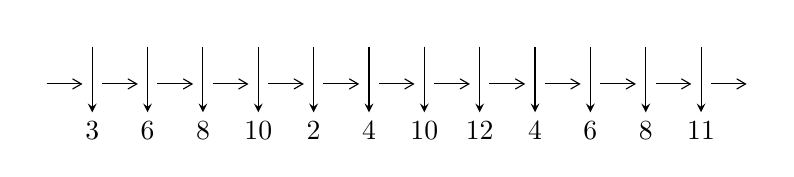
\begin{tikzpicture}[x=20pt, y=17pt]
	% nodes
	\node (C0) at (0, 0) {};
	\node (C1) at (1, 0) {};
	\node (C1U) at (1, +1) {};
	\node (C1D) at (1, -1) {3};

	\node (C2) at (2, 0) {};
	\node (C2U) at (2, +1) {};
	\node (C2D) at (2, -1) {6};

	\node (C3) at (3, 0) {};
	\node (C3U) at (3, +1) {};
	\node (C3D) at (3, -1) {8};

	\node (C4) at (4, 0) {};
	\node (C4U) at (4, +1) {};
	\node (C4D) at (4, -1) {10};

	\node (C5) at (5, 0) {};
	\node (C5U) at (5, +1) {};
	\node (C5D) at (5, -1) {2};

	\node (C6) at (6, 0) {};
	\node (C6U) at (6, +1) {};
	\node (C6D) at (6, -1) {4};

	\node (C7) at (7, 0) {};
	\node (C7U) at (7, +1) {};
	\node (C7D) at (7, -1) {10};

	\node (C8) at (8, 0) {};
	\node (C8U) at (8, +1) {};
	\node (C8D) at (8, -1) {12};

	\node (C9) at (9, 0) {};
	\node (C9U) at (9, +1) {};
	\node (C9D) at (9, -1) {4};

	\node (C10) at (10, 0) {};
	\node (C10U) at (10, +1) {};
	\node (C10D) at (10, -1) {6};

	\node (C11) at (11, 0) {};
	\node (C11U) at (11, +1) {};
	\node (C11D) at (11, -1) {8};

	\node (C12) at (12, 0) {};
	\node (C12U) at (12, +1) {};
	\node (C12D) at (12, -1) {11};
	\node (C13) at (13, 0) {};

	% arrows
	\draw[->,>={angle 60}]
	(C0) edge (C1) (C1) edge (C2) (C2) edge (C3) (C3) edge (C4) (C4) edge (C5) (C5) edge (C6) (C6) edge (C7) (C7) edge (C8) (C8) edge (C9) (C9) edge (C10) (C10) edge (C11) (C11) edge (C12) (C12) edge (C13) ;	\draw[->,>=stealth]
	(C1U) edge (C1D) (C2U) edge (C2D) (C3U) edge (C3D) (C4U) edge (C4D) (C5U) edge (C5D) (C6U) edge (C6D) (C7U) edge (C7D) (C8U) edge (C8D) (C9U) edge (C9D) (C10U) edge (C10D) (C11U) edge (C11D) (C12U) edge (C12D) ;
	\end{tikzpicture} \\
\hhline{~~} \\& 
\textbf{Solving Sequence} \\ \cline{2-2} 
 &
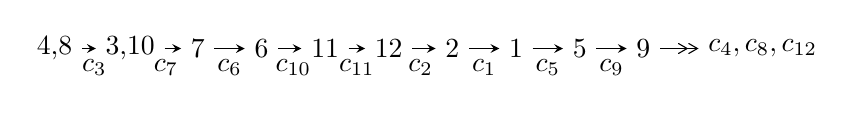
\begin{tikzpicture}[x=23pt, y=7pt]
	% node
	\node (A0) at (-1/8, 0) {4,8};
	\node (A1) at (17/16, 0) {3,10};
	\node (A2) at (17/8, 0) {7};
	\node (A3) at (25/8, 0) {6};
	\node (A4) at (33/8, 0) {11};
	\node (A5) at (41/8, 0) {12};
	\node (A6) at (49/8, 0) {2};
	\node (A7) at (57/8, 0) {1};
	\node (A8) at (65/8, 0) {5};
	\node (A9) at (73/8, 0) {9};
	\node (C1) at (1/2, -1) {$c_{3}$};
	\node (C2) at (13/8, -1) {$c_{7}$};
	\node (C3) at (21/8, -1) {$c_{6}$};
	\node (C4) at (29/8, -1) {$c_{10}$};
	\node (C5) at (37/8, -1) {$c_{11}$};
	\node (C6) at (45/8, -1) {$c_{2}$};
	\node (C7) at (53/8, -1) {$c_{1}$};
	\node (C8) at (61/8, -1) {$c_{5}$};
	\node (C9) at (69/8, -1) {$c_{9}$};
	\node (A10) at (11, 0) {$c_{4},c_{8},c_{12}$};

	% edge
	\draw[->,>=stealth]	
	(A0) edge (A1) (A1) edge (A2) (A2) edge (A3) (A3) edge (A4) (A4) edge (A5) (A5) edge (A6) (A6) edge (A7) (A7) edge (A8) (A8) edge (A9) ;
	\draw[->>,>={angle 60}]	
	(A9) edge (A10);
\end{tikzpicture} \\ 

\end{tabular} \\

\footnotetext{
The image of knot diagram is generated by the software ``\textbf{Draw programme}" developed by Andrew Bartholomew(\url{http://www.layer8.co.uk/maths/draw/index.htm\#Running-draw}), where we modified some parts for our purpose(\url{https://github.com/CATsTAILs/LinksPainter}).
}\phantom \\ \newline 
\centering \textbf{Ideals for irreducible components\footnotemark of $X_{\text{par}}$} 
 
\begin{align*}
I^u_{1}&=\langle 
-4283194 u^{11}+2308461 u^{10}+\cdots+21359143 b-4337843,\\
\phantom{I^u_{1}}&\phantom{= \langle  }-139682999 u^{11}+35486115 u^{10}+\cdots+21359143 a-526213370,\\
\phantom{I^u_{1}}&\phantom{= \langle  }u^{12}+u^{10}+10 u^9+u^8-6 u^7-28 u^6-45 u^5-26 u^4-34 u^3-3 u^2+5 u+1\rangle \\
I^u_{2}&=\langle 
- u^5-2 u^4- u^3-5 u^2+2 b+1,\;- u^5+u^4+4 u^3-2 u^2+4 a+13 u-3,\;u^6+2 u^5+u^4+4 u^3- u^2-2 u-1\rangle \\
I^u_{3}&=\langle 
u^2+b,\;- u^2+a+u+1,\;u^3- u^2-2 u+1\rangle \\
I^u_{4}&=\langle 
u^3+u^2+6 b+3 u+1,\;-2 u^3-23 u^2+138 a+30 u-77,\;u^4+8 u^2+4 u+23\rangle \\
I^u_{5}&=\langle 
b-1,\;a^2+a+1,\;u-1\rangle \\
\\
\end{align*}
\raggedright * 5 irreducible components of $\dim_{\mathbb{C}}=0$, with total 27 representations.\\
\footnotetext{All coefficients of polynomials are rational numbers. But the coefficients are sometimes approximated in decimal forms when there is not enough margin.}
\newpage
\renewcommand{\arraystretch}{1}
\centering \section*{I. $I^u_{1}= \langle -4.28\times10^{6} u^{11}+2.31\times10^{6} u^{10}+\cdots+2.14\times10^{7} b-4.34\times10^{6},\;-1.40\times10^{8} u^{11}+3.55\times10^{7} u^{10}+\cdots+2.14\times10^{7} a-5.26\times10^{8},\;u^{12}+u^{10}+\cdots+5 u+1 \rangle$}
\flushleft \textbf{(i) Arc colorings}\\
\begin{tabular}{m{7pt} m{180pt} m{7pt} m{180pt} }
\flushright $a_{4}=$&$\begin{pmatrix}1\\0\end{pmatrix}$ \\
\flushright $a_{8}=$&$\begin{pmatrix}0\\u\end{pmatrix}$ \\
\flushright $a_{3}=$&$\begin{pmatrix}1\\- u^2\end{pmatrix}$ \\
\flushright $a_{10}=$&$\begin{pmatrix}6.53973 u^{11}-1.66140 u^{10}+\cdots+29.8803 u+24.6364\\0.200532 u^{11}-0.108078 u^{10}+\cdots+3.23080 u+0.203091\end{pmatrix}$ \\
\flushright $a_{7}=$&$\begin{pmatrix}-9.40115 u^{11}+2.69041 u^{10}+\cdots-50.5716 u-32.5778\\1.66140 u^{11}-0.430541 u^{10}+\cdots+8.06220 u+6.53973\end{pmatrix}$ \\
\flushright $a_{6}=$&$\begin{pmatrix}-7.73975 u^{11}+2.25987 u^{10}+\cdots-42.5094 u-26.0381\\1.66140 u^{11}-0.430541 u^{10}+\cdots+8.06220 u+6.53973\end{pmatrix}$ \\
\flushright $a_{11}=$&$\begin{pmatrix}4.27986 u^{11}-1.02645 u^{10}+\cdots+17.2197 u+16.8967\\0.631073 u^{11}-0.239539 u^{10}+\cdots+4.99808 u+1.86449\end{pmatrix}$ \\
\flushright $a_{12}=$&$\begin{pmatrix}4.27986 u^{11}-1.02645 u^{10}+\cdots+17.2197 u+16.8967\\0.874490 u^{11}-0.282949 u^{10}+\cdots+5.85047 u+2.89094\end{pmatrix}$ \\
\flushright $a_{2}=$&$\begin{pmatrix}4.87432 u^{11}-1.53943 u^{10}+\cdots+31.4054 u+15.7081\\-2.28293 u^{11}+0.628514 u^{10}+\cdots-11.6846 u-8.27969\end{pmatrix}$ \\
\flushright $a_{1}=$&$\begin{pmatrix}3.10484 u^{11}-1.07242 u^{10}+\cdots+22.5436 u+8.96784\\-2.13788 u^{11}+0.599560 u^{10}+\cdots-11.1190 u-7.81268\end{pmatrix}$ \\
\flushright $a_{5}=$&$\begin{pmatrix}-6.53973 u^{11}+1.66140 u^{10}+\cdots-29.8803 u-24.6364\\-0.641879 u^{11}+0.236936 u^{10}+\cdots-4.78908 u-1.44344\end{pmatrix}$ \\
\flushright $a_{9}=$&$\begin{pmatrix}6.74026 u^{11}-1.76948 u^{10}+\cdots+33.1111 u+24.8395\\0.200532 u^{11}-0.108078 u^{10}+\cdots+3.23080 u+0.203091\end{pmatrix}$\\&\end{tabular}
\flushleft \textbf{(ii) Obstruction class $= -1$}\\~\\
\flushleft \textbf{(iii) Cusp Shapes $= \frac{16757967}{1643011} u^{11}-\frac{5020278}{1643011} u^{10}+\cdots+\frac{1299731}{23141} u+\frac{33667882}{1643011}$}\\~\\
\newpage\renewcommand{\arraystretch}{1}
\flushleft \textbf{(iv) u-Polynomials at the component}\newline \\
\begin{tabular}{m{50pt}|m{274pt}}
Crossings & \hspace{64pt}u-Polynomials at each crossing \\
\hline $$\begin{aligned}c_{1},c_{12}\end{aligned}$$&$\begin{aligned}
&u^{12}+11 u^{11}+\cdots+22 u+1
\end{aligned}$\\
\hline $$\begin{aligned}c_{2},c_{5},c_{8}\\c_{11}\end{aligned}$$&$\begin{aligned}
&u^{12}+u^{11}+\cdots-2 u-1
\end{aligned}$\\
\hline $$\begin{aligned}c_{3},c_{10}\end{aligned}$$&$\begin{aligned}
&u^{12}+u^{10}+\cdots-5 u+1
\end{aligned}$\\
\hline $$\begin{aligned}c_{4},c_{9}\end{aligned}$$&$\begin{aligned}
&u^{12}-4 u^{11}+\cdots+3 u+1
\end{aligned}$\\
\hline $$\begin{aligned}c_{6},c_{7}\end{aligned}$$&$\begin{aligned}
&u^{12}- u^{11}+\cdots+2 u+1
\end{aligned}$\\
\hline
\end{tabular}\\~\\
\newpage\renewcommand{\arraystretch}{1}
\flushleft \textbf{(v) Riley Polynomials at the component}\newline \\
\begin{tabular}{m{50pt}|m{274pt}}
Crossings & \hspace{64pt}Riley Polynomials at each crossing \\
\hline $$\begin{aligned}c_{1},c_{12}\end{aligned}$$&$\begin{aligned}
&y^{12}-11 y^{11}+\cdots-154 y+1
\end{aligned}$\\
\hline $$\begin{aligned}c_{2},c_{5},c_{8}\\c_{11}\end{aligned}$$&$\begin{aligned}
&y^{12}-11 y^{11}+\cdots-22 y+1
\end{aligned}$\\
\hline $$\begin{aligned}c_{3},c_{10}\end{aligned}$$&$\begin{aligned}
&y^{12}+2 y^{11}+\cdots-31 y+1
\end{aligned}$\\
\hline $$\begin{aligned}c_{4},c_{9}\end{aligned}$$&$\begin{aligned}
&y^{12}-30 y^{11}+\cdots+45 y+1
\end{aligned}$\\
\hline $$\begin{aligned}c_{6},c_{7}\end{aligned}$$&$\begin{aligned}
&y^{12}-7 y^{11}+\cdots-14 y+1
\end{aligned}$\\
\hline
\end{tabular}\\~\\
\newpage\flushleft \textbf{(vi) Complex Volumes and Cusp Shapes}
$$\begin{array}{c|c|c}  
\text{Solutions to }I^u_{1}& \I (\text{vol} + \sqrt{-1}CS) & \text{Cusp shape}\\
 \hline 
\begin{aligned}
u &= \phantom{-}0.141786 + 0.980425 I \\
a &= -0.933540 + 0.158952 I \\
b &= \phantom{-}0.041012 + 0.177252 I\end{aligned}
 & \phantom{-}1.74171 - 4.08194 I & -5.82114 + 7.56540 I \\ \hline\begin{aligned}
u &= \phantom{-}0.141786 - 0.980425 I \\
a &= -0.933540 - 0.158952 I \\
b &= \phantom{-}0.041012 - 0.177252 I\end{aligned}
 & \phantom{-}1.74171 + 4.08194 I & -5.82114 - 7.56540 I \\ \hline\begin{aligned}
u &= -0.442926 + 1.140420 I \\
a &= -0.476761 + 0.082105 I \\
b &= \phantom{-}1.037070 + 0.350813 I\end{aligned}
 & -1.35590 + 2.26651 I & -17.0173 - 3.2135 I \\ \hline\begin{aligned}
u &= -0.442926 - 1.140420 I \\
a &= -0.476761 - 0.082105 I \\
b &= \phantom{-}1.037070 - 0.350813 I\end{aligned}
 & -1.35590 - 2.26651 I & -17.0173 + 3.2135 I \\ \hline\begin{aligned}
u &= -1.29341\phantom{ +0.000000I} \\
a &= \phantom{-}1.70253\phantom{ +0.000000I} \\
b &= -1.58736\phantom{ +0.000000I}\end{aligned}
 & -7.73551\phantom{ +0.000000I} & -2.14220\phantom{ +0.000000I} \\ \hline\begin{aligned}
u &= \phantom{-}0.362550\phantom{ +0.000000I} \\
a &= -0.697529\phantom{ +0.000000I} \\
b &= \phantom{-}0.433632\phantom{ +0.000000I}\end{aligned}
 & -0.619674\phantom{ +0.000000I} & -15.7990\phantom{ +0.000000I} \\ \hline\begin{aligned}
u &= \phantom{-}1.68235\phantom{ +0.000000I} \\
a &= \phantom{-}1.15411\phantom{ +0.000000I} \\
b &= -1.86647\phantom{ +0.000000I}\end{aligned}
 & -12.8318\phantom{ +0.000000I} & -20.4330\phantom{ +0.000000I} \\ \hline\begin{aligned}
u &= -0.277013 + 0.027736 I \\
a &= \phantom{-}2.61966 + 3.59517 I \\
b &= -1.132390 + 0.181685 I\end{aligned}
 & -1.88495 - 4.13308 I & -16.9007 + 5.9544 I \\ \hline\begin{aligned}
u &= -0.277013 - 0.027736 I \\
a &= \phantom{-}2.61966 - 3.59517 I \\
b &= -1.132390 - 0.181685 I\end{aligned}
 & -1.88495 + 4.13308 I & -16.9007 - 5.9544 I \\ \hline\begin{aligned}
u &= -1.90708\phantom{ +0.000000I} \\
a &= -0.231901\phantom{ +0.000000I} \\
b &= \phantom{-}3.31219\phantom{ +0.000000I}\end{aligned}
 & -18.8402\phantom{ +0.000000I} & -5.38040\phantom{ +0.000000I}\\
 \hline 
 \end{array}$$\newpage$$\begin{array}{c|c|c}  
\text{Solutions to }I^u_{1}& \I (\text{vol} + \sqrt{-1}CS) & \text{Cusp shape}\\
 \hline 
\begin{aligned}
u &= \phantom{-}1.15595 + 2.12191 I \\
a &= \phantom{-}0.827033 - 0.271266 I \\
b &= -2.09169 - 0.35807 I\end{aligned}
 & \phantom{-}4.24091 - 10.44050 I & -12.38352 + 4.77186 I \\ \hline\begin{aligned}
u &= \phantom{-}1.15595 - 2.12191 I \\
a &= \phantom{-}0.827033 + 0.271266 I \\
b &= -2.09169 + 0.35807 I\end{aligned}
 & \phantom{-}4.24091 + 10.44050 I & -12.38352 - 4.77186 I\\
 \hline 
 \end{array}$$\newpage\newpage\renewcommand{\arraystretch}{1}
\centering \section*{II. $I^u_{2}= \langle - u^5-2 u^4- u^3-5 u^2+2 b+1,\;- u^5+u^4+4 u^3-2 u^2+4 a+13 u-3,\;u^6+2 u^5+u^4+4 u^3- u^2-2 u-1 \rangle$}
\flushleft \textbf{(i) Arc colorings}\\
\begin{tabular}{m{7pt} m{180pt} m{7pt} m{180pt} }
\flushright $a_{4}=$&$\begin{pmatrix}1\\0\end{pmatrix}$ \\
\flushright $a_{8}=$&$\begin{pmatrix}0\\u\end{pmatrix}$ \\
\flushright $a_{3}=$&$\begin{pmatrix}1\\- u^2\end{pmatrix}$ \\
\flushright $a_{10}=$&$\begin{pmatrix}\frac{1}{4} u^5-\frac{1}{4} u^4+\cdots-\frac{13}{4} u+\frac{3}{4}\\\frac{1}{2} u^5+u^4+\frac{1}{2} u^3+\frac{5}{2} u^2-\frac{1}{2}\end{pmatrix}$ \\
\flushright $a_{7}=$&$\begin{pmatrix}-\frac{5}{4} u^5-\frac{7}{4} u^4+\cdots+\frac{19}{4} u+\frac{11}{4}\\-\frac{1}{4} u^5-\frac{3}{4} u^4+\cdots-\frac{3}{4} u+\frac{1}{4}\end{pmatrix}$ \\
\flushright $a_{6}=$&$\begin{pmatrix}-\frac{3}{2} u^5-\frac{5}{2} u^4+\cdots+4 u+3\\-\frac{1}{4} u^5-\frac{3}{4} u^4+\cdots-\frac{3}{4} u+\frac{1}{4}\end{pmatrix}$ \\
\flushright $a_{11}=$&$\begin{pmatrix}\frac{1}{4} u^5+\frac{3}{4} u^4+\cdots+\frac{5}{4} u-\frac{7}{4}\\-\frac{1}{4} u^5-\frac{3}{4} u^4+\cdots-\frac{3}{4} u-\frac{3}{4}\end{pmatrix}$ \\
\flushright $a_{12}=$&$\begin{pmatrix}\frac{1}{4} u^5+\frac{3}{4} u^4+\cdots+\frac{5}{4} u-\frac{7}{4}\\-\frac{1}{2} u^5- u^4-\frac{1}{2} u^3-\frac{5}{2} u^2-\frac{1}{2}\end{pmatrix}$ \\
\flushright $a_{2}=$&$\begin{pmatrix}2 u^5+\frac{7}{2} u^4+u^3+8 u^2-3 u-\frac{5}{2}\\-\frac{1}{4} u^5-\frac{3}{4} u^4+\cdots-\frac{3}{4} u-\frac{3}{4}\end{pmatrix}$ \\
\flushright $a_{1}=$&$\begin{pmatrix}\frac{7}{4} u^5+\frac{13}{4} u^4+\cdots-\frac{11}{4} u-\frac{15}{4}\\- u^2- u-1\end{pmatrix}$ \\
\flushright $a_{5}=$&$\begin{pmatrix}\frac{1}{4} u^5+\frac{1}{4} u^4+\cdots-\frac{7}{4} u-\frac{5}{4}\\\frac{1}{2} u^4+u^3+u^2+2 u+\frac{1}{2}\end{pmatrix}$ \\
\flushright $a_{9}=$&$\begin{pmatrix}\frac{3}{4} u^5+\frac{3}{4} u^4+\cdots-\frac{13}{4} u+\frac{1}{4}\\\frac{1}{2} u^5+u^4+\frac{1}{2} u^3+\frac{5}{2} u^2-\frac{1}{2}\end{pmatrix}$\\&\end{tabular}
\flushleft \textbf{(ii) Obstruction class $= 1$}\\~\\
\flushleft \textbf{(iii) Cusp Shapes $= u^5+\frac{3}{2} u^4+4 u^2-2 u-\frac{25}{2}$}\\~\\
\newpage\renewcommand{\arraystretch}{1}
\flushleft \textbf{(iv) u-Polynomials at the component}\newline \\
\begin{tabular}{m{50pt}|m{274pt}}
Crossings & \hspace{64pt}u-Polynomials at each crossing \\
\hline $$\begin{aligned}c_{1}\end{aligned}$$&$\begin{aligned}
&u^6-5 u^5+10 u^4-13 u^3+14 u^2-9 u+1
\end{aligned}$\\
\hline $$\begin{aligned}c_{2},c_{8}\end{aligned}$$&$\begin{aligned}
&u^6+u^5-2 u^4-3 u^3+3 u+1
\end{aligned}$\\
\hline $$\begin{aligned}c_{3}\end{aligned}$$&$\begin{aligned}
&u^6+2 u^5+u^4+4 u^3- u^2-2 u-1
\end{aligned}$\\
\hline $$\begin{aligned}c_{4}\end{aligned}$$&$\begin{aligned}
&(u^3- u^2- u-1)^2
\end{aligned}$\\
\hline $$\begin{aligned}c_{5},c_{11}\end{aligned}$$&$\begin{aligned}
&u^6- u^5-2 u^4+3 u^3-3 u+1
\end{aligned}$\\
\hline $$\begin{aligned}c_{6}\end{aligned}$$&$\begin{aligned}
&u^6+u^5-2 u^4-5 u^3-8 u^2-5 u-1
\end{aligned}$\\
\hline $$\begin{aligned}c_{7}\end{aligned}$$&$\begin{aligned}
&u^6- u^5-2 u^4+5 u^3-8 u^2+5 u-1
\end{aligned}$\\
\hline $$\begin{aligned}c_{9}\end{aligned}$$&$\begin{aligned}
&(u^3+u^2- u+1)^2
\end{aligned}$\\
\hline $$\begin{aligned}c_{10}\end{aligned}$$&$\begin{aligned}
&u^6-2 u^5+u^4-4 u^3- u^2+2 u-1
\end{aligned}$\\
\hline $$\begin{aligned}c_{12}\end{aligned}$$&$\begin{aligned}
&u^6+5 u^5+10 u^4+13 u^3+14 u^2+9 u+1
\end{aligned}$\\
\hline
\end{tabular}\\~\\
\newpage\renewcommand{\arraystretch}{1}
\flushleft \textbf{(v) Riley Polynomials at the component}\newline \\
\begin{tabular}{m{50pt}|m{274pt}}
Crossings & \hspace{64pt}Riley Polynomials at each crossing \\
\hline $$\begin{aligned}c_{1},c_{12}\end{aligned}$$&$\begin{aligned}
&y^6-5 y^5-2 y^4+23 y^3-18 y^2-53 y+1
\end{aligned}$\\
\hline $$\begin{aligned}c_{2},c_{5},c_{8}\\c_{11}\end{aligned}$$&$\begin{aligned}
&y^6-5 y^5+10 y^4-13 y^3+14 y^2-9 y+1
\end{aligned}$\\
\hline $$\begin{aligned}c_{3},c_{10}\end{aligned}$$&$\begin{aligned}
&y^6-2 y^5-17 y^4-12 y^3+15 y^2-2 y+1
\end{aligned}$\\
\hline $$\begin{aligned}c_{4},c_{9}\end{aligned}$$&$\begin{aligned}
&(y^3-3 y^2- y-1)^2
\end{aligned}$\\
\hline $$\begin{aligned}c_{6},c_{7}\end{aligned}$$&$\begin{aligned}
&y^6-5 y^5-2 y^4+15 y^3+18 y^2-9 y+1
\end{aligned}$\\
\hline
\end{tabular}\\~\\
\newpage\flushleft \textbf{(vi) Complex Volumes and Cusp Shapes}
$$\begin{array}{c|c|c}  
\text{Solutions to }I^u_{2}& \I (\text{vol} + \sqrt{-1}CS) & \text{Cusp shape}\\
 \hline 
\begin{aligned}
u &= \phantom{-}0.788614\phantom{ +0.000000I} \\
a &= -2.01293\phantom{ +0.000000I} \\
b &= \phantom{-}1.83929\phantom{ +0.000000I}\end{aligned}
 & -11.8065\phantom{ +0.000000I} & -10.7040\phantom{ +0.000000I} \\ \hline\begin{aligned}
u &= \phantom{-}0.15540 + 1.44647 I \\
a &= -0.005444 + 0.311582 I \\
b &= -0.419643 + 0.606291 I\end{aligned}
 & \phantom{-}0.96847 - 3.17729 I & -11.64780 + 1.72143 I \\ \hline\begin{aligned}
u &= \phantom{-}0.15540 - 1.44647 I \\
a &= -0.005444 - 0.311582 I \\
b &= -0.419643 - 0.606291 I\end{aligned}
 & \phantom{-}0.96847 + 3.17729 I & -11.64780 - 1.72143 I \\ \hline\begin{aligned}
u &= -0.383557 + 0.331324 I \\
a &= \phantom{-}1.96878 - 1.31241 I \\
b &= -0.419643 - 0.606291 I\end{aligned}
 & \phantom{-}0.96847 + 3.17729 I & -11.64780 - 1.72143 I \\ \hline\begin{aligned}
u &= -0.383557 - 0.331324 I \\
a &= \phantom{-}1.96878 + 1.31241 I \\
b &= -0.419643 + 0.606291 I\end{aligned}
 & \phantom{-}0.96847 - 3.17729 I & -11.64780 + 1.72143 I \\ \hline\begin{aligned}
u &= -2.33230\phantom{ +0.000000I} \\
a &= -0.913737\phantom{ +0.000000I} \\
b &= \phantom{-}1.83929\phantom{ +0.000000I}\end{aligned}
 & -11.8065\phantom{ +0.000000I} & -10.7040\phantom{ +0.000000I}\\
 \hline 
 \end{array}$$\newpage\newpage\renewcommand{\arraystretch}{1}
\centering \section*{III. $I^u_{3}= \langle u^2+b,\;- u^2+a+u+1,\;u^3- u^2-2 u+1 \rangle$}
\flushleft \textbf{(i) Arc colorings}\\
\begin{tabular}{m{7pt} m{180pt} m{7pt} m{180pt} }
\flushright $a_{4}=$&$\begin{pmatrix}1\\0\end{pmatrix}$ \\
\flushright $a_{8}=$&$\begin{pmatrix}0\\u\end{pmatrix}$ \\
\flushright $a_{3}=$&$\begin{pmatrix}1\\- u^2\end{pmatrix}$ \\
\flushright $a_{10}=$&$\begin{pmatrix}u^2- u-1\\- u^2\end{pmatrix}$ \\
\flushright $a_{7}=$&$\begin{pmatrix}- u^2+2 u\\- u+1\end{pmatrix}$ \\
\flushright $a_{6}=$&$\begin{pmatrix}- u^2+u+1\\- u+1\end{pmatrix}$ \\
\flushright $a_{11}=$&$\begin{pmatrix}u^2-2\\- u\end{pmatrix}$ \\
\flushright $a_{12}=$&$\begin{pmatrix}u^2-2\\u^2-1\end{pmatrix}$ \\
\flushright $a_{2}=$&$\begin{pmatrix}0\\- u^2- u\end{pmatrix}$ \\
\flushright $a_{1}=$&$\begin{pmatrix}- u^2- u\\3 u^2+2 u-2\end{pmatrix}$ \\
\flushright $a_{5}=$&$\begin{pmatrix}- u^2+u+1\\3 u^2+u-1\end{pmatrix}$ \\
\flushright $a_{9}=$&$\begin{pmatrix}- u-1\\- u^2\end{pmatrix}$\\&\end{tabular}
\flushleft \textbf{(ii) Obstruction class $= 1$}\\~\\
\flushleft \textbf{(iii) Cusp Shapes $= -5 u^2+6 u-19$}\\~\\
\newpage\renewcommand{\arraystretch}{1}
\flushleft \textbf{(iv) u-Polynomials at the component}\newline \\
\begin{tabular}{m{50pt}|m{274pt}}
Crossings & \hspace{64pt}u-Polynomials at each crossing \\
\hline $$\begin{aligned}c_{1}\end{aligned}$$&$\begin{aligned}
&u^3-6 u^2+5 u-1
\end{aligned}$\\
\hline $$\begin{aligned}c_{2},c_{6},c_{8}\end{aligned}$$&$\begin{aligned}
&u^3+2 u^2- u-1
\end{aligned}$\\
\hline $$\begin{aligned}c_{3}\end{aligned}$$&$\begin{aligned}
&u^3- u^2-2 u+1
\end{aligned}$\\
\hline $$\begin{aligned}c_{4}\end{aligned}$$&$\begin{aligned}
&u^3+5 u^2+6 u+1
\end{aligned}$\\
\hline $$\begin{aligned}c_{5},c_{7},c_{11}\end{aligned}$$&$\begin{aligned}
&u^3-2 u^2- u+1
\end{aligned}$\\
\hline $$\begin{aligned}c_{9}\end{aligned}$$&$\begin{aligned}
&u^3-5 u^2+6 u-1
\end{aligned}$\\
\hline $$\begin{aligned}c_{10}\end{aligned}$$&$\begin{aligned}
&u^3+u^2-2 u-1
\end{aligned}$\\
\hline $$\begin{aligned}c_{12}\end{aligned}$$&$\begin{aligned}
&u^3+6 u^2+5 u+1
\end{aligned}$\\
\hline
\end{tabular}\\~\\
\newpage\renewcommand{\arraystretch}{1}
\flushleft \textbf{(v) Riley Polynomials at the component}\newline \\
\begin{tabular}{m{50pt}|m{274pt}}
Crossings & \hspace{64pt}Riley Polynomials at each crossing \\
\hline $$\begin{aligned}c_{1},c_{12}\end{aligned}$$&$\begin{aligned}
&y^3-26 y^2+13 y-1
\end{aligned}$\\
\hline $$\begin{aligned}c_{2},c_{5},c_{6}\\c_{7},c_{8},c_{11}\end{aligned}$$&$\begin{aligned}
&y^3-6 y^2+5 y-1
\end{aligned}$\\
\hline $$\begin{aligned}c_{3},c_{10}\end{aligned}$$&$\begin{aligned}
&y^3-5 y^2+6 y-1
\end{aligned}$\\
\hline $$\begin{aligned}c_{4},c_{9}\end{aligned}$$&$\begin{aligned}
&y^3-13 y^2+26 y-1
\end{aligned}$\\
\hline
\end{tabular}\\~\\
\newpage\flushleft \textbf{(vi) Complex Volumes and Cusp Shapes}
$$\begin{array}{c|c|c}  
\text{Solutions to }I^u_{3}& \I (\text{vol} + \sqrt{-1}CS) & \text{Cusp shape}\\
 \hline 
\begin{aligned}
u &= -1.24698\phantom{ +0.000000I} \\
a &= \phantom{-}1.80194\phantom{ +0.000000I} \\
b &= -1.55496\phantom{ +0.000000I}\end{aligned}
 & -7.98968\phantom{ +0.000000I} & -34.2570\phantom{ +0.000000I} \\ \hline\begin{aligned}
u &= \phantom{-}0.445042\phantom{ +0.000000I} \\
a &= -1.24698\phantom{ +0.000000I} \\
b &= -0.198062\phantom{ +0.000000I}\end{aligned}
 & -2.34991\phantom{ +0.000000I} & -17.3200\phantom{ +0.000000I} \\ \hline\begin{aligned}
u &= \phantom{-}1.80194\phantom{ +0.000000I} \\
a &= \phantom{-}0.445042\phantom{ +0.000000I} \\
b &= -3.24698\phantom{ +0.000000I}\end{aligned}
 & -19.2692\phantom{ +0.000000I} & -24.4230\phantom{ +0.000000I}\\
 \hline 
 \end{array}$$\newpage\newpage\renewcommand{\arraystretch}{1}
\centering \section*{IV. $I^u_{4}= \langle u^3+u^2+6 b+3 u+1,\;-2 u^3-23 u^2+138 a+30 u-77,\;u^4+8 u^2+4 u+23 \rangle$}
\flushleft \textbf{(i) Arc colorings}\\
\begin{tabular}{m{7pt} m{180pt} m{7pt} m{180pt} }
\flushright $a_{4}=$&$\begin{pmatrix}1\\0\end{pmatrix}$ \\
\flushright $a_{8}=$&$\begin{pmatrix}0\\u\end{pmatrix}$ \\
\flushright $a_{3}=$&$\begin{pmatrix}1\\- u^2\end{pmatrix}$ \\
\flushright $a_{10}=$&$\begin{pmatrix}\frac{1}{69} u^3+\frac{1}{6} u^2-\frac{5}{23} u+\frac{77}{138}\\-\frac{1}{6} u^3-\frac{1}{6} u^2-\frac{1}{2} u-\frac{1}{6}\end{pmatrix}$ \\
\flushright $a_{7}=$&$\begin{pmatrix}0.0507246 u^{3}+0.333333 u^{2}+0.239130 u+2.20290\\-\frac{1}{2} u^2-\frac{5}{2}\end{pmatrix}$ \\
\flushright $a_{6}=$&$\begin{pmatrix}0.0507246 u^{3}-0.166667 u^{2}+0.239130 u-0.297101\\-\frac{1}{2} u^2-\frac{5}{2}\end{pmatrix}$ \\
\flushright $a_{11}=$&$\begin{pmatrix}-\frac{3}{46} u^3-\frac{1}{46} u-\frac{6}{23}\\-\frac{2}{3} u^3-\frac{1}{6} u^2-2 u-\frac{7}{6}\end{pmatrix}$ \\
\flushright $a_{12}=$&$\begin{pmatrix}-\frac{3}{46} u^3-\frac{1}{46} u-\frac{6}{23}\\-\frac{1}{6} u^3-\frac{1}{6} u^2-\frac{1}{2} u-\frac{7}{6}\end{pmatrix}$ \\
\flushright $a_{2}=$&$\begin{pmatrix}\frac{1}{23} u^3+\frac{8}{23} u+\frac{4}{23}\\-\frac{1}{2} u^2-\frac{1}{2}\end{pmatrix}$ \\
\flushright $a_{1}=$&$\begin{pmatrix}\frac{1}{23} u^3-\frac{1}{2} u^2-\frac{15}{23} u-\frac{15}{46}\\u^3-4 u^2-2 u-12\end{pmatrix}$ \\
\flushright $a_{5}=$&$\begin{pmatrix}\frac{5}{46} u^3+\frac{17}{46} u+\frac{10}{23}\\-\frac{1}{3} u^3-\frac{1}{3} u^2- u+\frac{2}{3}\end{pmatrix}$ \\
\flushright $a_{9}=$&$\begin{pmatrix}-\frac{7}{46} u^3-\frac{33}{46} u+\frac{9}{23}\\-\frac{1}{6} u^3-\frac{1}{6} u^2-\frac{1}{2} u-\frac{1}{6}\end{pmatrix}$\\&\end{tabular}
\flushleft \textbf{(ii) Obstruction class $= -1$}\\~\\
\flushleft \textbf{(iii) Cusp Shapes $= -10$}\\~\\
\newpage\renewcommand{\arraystretch}{1}
\flushleft \textbf{(iv) u-Polynomials at the component}\newline \\
\begin{tabular}{m{50pt}|m{274pt}}
Crossings & \hspace{64pt}u-Polynomials at each crossing \\
\hline $$\begin{aligned}c_{1},c_{12}\end{aligned}$$&$\begin{aligned}
&u^4-6 u^3+31 u^2-66 u+49
\end{aligned}$\\
\hline $$\begin{aligned}c_{2},c_{5},c_{8}\\c_{11}\end{aligned}$$&$\begin{aligned}
&u^4+2 u^3+5 u^2+2 u+7
\end{aligned}$\\
\hline $$\begin{aligned}c_{3},c_{10}\end{aligned}$$&$\begin{aligned}
&u^4+8 u^2-4 u+23
\end{aligned}$\\
\hline $$\begin{aligned}c_{4},c_{9}\end{aligned}$$&$\begin{aligned}
&(u^2+2 u-1)^2
\end{aligned}$\\
\hline $$\begin{aligned}c_{6},c_{7}\end{aligned}$$&$\begin{aligned}
&u^4-2 u^3+5 u^2-6 u+9
\end{aligned}$\\
\hline
\end{tabular}\\~\\
\newpage\renewcommand{\arraystretch}{1}
\flushleft \textbf{(v) Riley Polynomials at the component}\newline \\
\begin{tabular}{m{50pt}|m{274pt}}
Crossings & \hspace{64pt}Riley Polynomials at each crossing \\
\hline $$\begin{aligned}c_{1},c_{12}\end{aligned}$$&$\begin{aligned}
&y^4+26 y^3+267 y^2-1318 y+2401
\end{aligned}$\\
\hline $$\begin{aligned}c_{2},c_{5},c_{8}\\c_{11}\end{aligned}$$&$\begin{aligned}
&y^4+6 y^3+31 y^2+66 y+49
\end{aligned}$\\
\hline $$\begin{aligned}c_{3},c_{10}\end{aligned}$$&$\begin{aligned}
&y^4+16 y^3+110 y^2+352 y+529
\end{aligned}$\\
\hline $$\begin{aligned}c_{4},c_{9}\end{aligned}$$&$\begin{aligned}
&(y^2-6 y+1)^2
\end{aligned}$\\
\hline $$\begin{aligned}c_{6},c_{7}\end{aligned}$$&$\begin{aligned}
&y^4+6 y^3+19 y^2+54 y+81
\end{aligned}$\\
\hline
\end{tabular}\\~\\
\newpage\flushleft \textbf{(vi) Complex Volumes and Cusp Shapes}
$$\begin{array}{c|c|c}  
\text{Solutions to }I^u_{4}& \I (\text{vol} + \sqrt{-1}CS) & \text{Cusp shape}\\
 \hline 
\begin{aligned}
u &= -0.70711 + 1.75664 I \\
a &= \phantom{-}0.370470 - 0.836294 I \\
b &= -0.414214\phantom{ +0.000000I}\end{aligned}
 & \phantom{-}4.93480\phantom{ +0.000000I} & -10.0000\phantom{ +0.000000I} \\ \hline\begin{aligned}
u &= -0.70711 - 1.75664 I \\
a &= \phantom{-}0.370470 + 0.836294 I \\
b &= -0.414214\phantom{ +0.000000I}\end{aligned}
 & \phantom{-}4.93480\phantom{ +0.000000I} & -10.0000\phantom{ +0.000000I} \\ \hline\begin{aligned}
u &= \phantom{-}0.70711 + 2.43192 I \\
a &= -0.674818 - 0.111049 I \\
b &= \phantom{-}2.41421\phantom{ +0.000000I}\end{aligned}
 & \phantom{-}4.93480\phantom{ +0.000000I} & -10.0000\phantom{ +0.000000I} \\ \hline\begin{aligned}
u &= \phantom{-}0.70711 - 2.43192 I \\
a &= -0.674818 + 0.111049 I \\
b &= \phantom{-}2.41421\phantom{ +0.000000I}\end{aligned}
 & \phantom{-}4.93480\phantom{ +0.000000I} & -10.0000\phantom{ +0.000000I}\\
 \hline 
 \end{array}$$\newpage\newpage\renewcommand{\arraystretch}{1}
\centering \section*{V. $I^u_{5}= \langle b-1,\;a^2+a+1,\;u-1 \rangle$}
\flushleft \textbf{(i) Arc colorings}\\
\begin{tabular}{m{7pt} m{180pt} m{7pt} m{180pt} }
\flushright $a_{4}=$&$\begin{pmatrix}1\\0\end{pmatrix}$ \\
\flushright $a_{8}=$&$\begin{pmatrix}0\\1\end{pmatrix}$ \\
\flushright $a_{3}=$&$\begin{pmatrix}1\\-1\end{pmatrix}$ \\
\flushright $a_{10}=$&$\begin{pmatrix}a\\1\end{pmatrix}$ \\
\flushright $a_{7}=$&$\begin{pmatrix}- a-1\\a+1\end{pmatrix}$ \\
\flushright $a_{6}=$&$\begin{pmatrix}0\\a+1\end{pmatrix}$ \\
\flushright $a_{11}=$&$\begin{pmatrix}a\\- a\end{pmatrix}$ \\
\flushright $a_{12}=$&$\begin{pmatrix}a\\0\end{pmatrix}$ \\
\flushright $a_{2}=$&$\begin{pmatrix}1\\- a-1\end{pmatrix}$ \\
\flushright $a_{1}=$&$\begin{pmatrix}- a+1\\-1\end{pmatrix}$ \\
\flushright $a_{5}=$&$\begin{pmatrix}a+1\\1\end{pmatrix}$ \\
\flushright $a_{9}=$&$\begin{pmatrix}a+1\\1\end{pmatrix}$\\&\end{tabular}
\flushleft \textbf{(ii) Obstruction class $= -1$}\\~\\
\flushleft \textbf{(iii) Cusp Shapes $= -12$}\\~\\
\newpage\renewcommand{\arraystretch}{1}
\flushleft \textbf{(iv) u-Polynomials at the component}\newline \\
\begin{tabular}{m{50pt}|m{274pt}}
Crossings & \hspace{64pt}u-Polynomials at each crossing \\
\hline $$\begin{aligned}c_{1},c_{12}\end{aligned}$$&$\begin{aligned}
&u^2- u+1
\end{aligned}$\\
\hline $$\begin{aligned}c_{2},c_{5},c_{6}\\c_{7},c_{8},c_{11}\end{aligned}$$&$\begin{aligned}
&u^2+u+1
\end{aligned}$\\
\hline $$\begin{aligned}c_{3},c_{4},c_{9}\\c_{10}\end{aligned}$$&$\begin{aligned}
&(u+1)^2
\end{aligned}$\\
\hline
\end{tabular}\\~\\
\newpage\renewcommand{\arraystretch}{1}
\flushleft \textbf{(v) Riley Polynomials at the component}\newline \\
\begin{tabular}{m{50pt}|m{274pt}}
Crossings & \hspace{64pt}Riley Polynomials at each crossing \\
\hline $$\begin{aligned}c_{1},c_{2},c_{5}\\c_{6},c_{7},c_{8}\\c_{11},c_{12}\end{aligned}$$&$\begin{aligned}
&y^2+y+1
\end{aligned}$\\
\hline $$\begin{aligned}c_{3},c_{4},c_{9}\\c_{10}\end{aligned}$$&$\begin{aligned}
&(y-1)^2
\end{aligned}$\\
\hline
\end{tabular}\\~\\
\newpage\flushleft \textbf{(vi) Complex Volumes and Cusp Shapes}
$$\begin{array}{c|c|c}  
\text{Solutions to }I^u_{5}& \I (\text{vol} + \sqrt{-1}CS) & \text{Cusp shape}\\
 \hline 
\begin{aligned}
u &= \phantom{-}1.00000\phantom{ +0.000000I} \\
a &= -0.500000 + 0.866025 I \\
b &= \phantom{-}1.00000\phantom{ +0.000000I}\end{aligned}
 & \phantom{-0.000000 } 0 & -12.0000\phantom{ +0.000000I} \\ \hline\begin{aligned}
u &= \phantom{-}1.00000\phantom{ +0.000000I} \\
a &= -0.500000 - 0.866025 I \\
b &= \phantom{-}1.00000\phantom{ +0.000000I}\end{aligned}
 & \phantom{-0.000000 } 0 & -12.0000\phantom{ +0.000000I}\\
 \hline 
 \end{array}$$\newpage
\newpage\renewcommand{\arraystretch}{1}
\centering \section*{ VI. u-Polynomials}
\begin{tabular}{m{50pt}|m{274pt}}
Crossings & \hspace{64pt}u-Polynomials at each crossing \\
\hline $$\begin{aligned}c_{1}\end{aligned}$$&$\begin{aligned}
&(u^2- u+1)(u^3-6 u^2+5 u-1)(u^4-6 u^3+31 u^2-66 u+49)\\
&\cdot(u^6-5 u^5+\cdots-9 u+1)(u^{12}+11 u^{11}+\cdots+22 u+1)
\end{aligned}$\\
\hline $$\begin{aligned}c_{2},c_{8}\end{aligned}$$&$\begin{aligned}
&(u^2+u+1)(u^3+2 u^2- u-1)(u^4+2 u^3+5 u^2+2 u+7)\\
&\cdot(u^6+u^5-2 u^4-3 u^3+3 u+1)(u^{12}+u^{11}+\cdots-2 u-1)
\end{aligned}$\\
\hline $$\begin{aligned}c_{3}\end{aligned}$$&$\begin{aligned}
&(u+1)^2(u^3- u^2-2 u+1)(u^4+8 u^2-4 u+23)\\
&\cdot(u^6+2 u^5+u^4+4 u^3- u^2-2 u-1)(u^{12}+u^{10}+\cdots-5 u+1)
\end{aligned}$\\
\hline $$\begin{aligned}c_{4}\end{aligned}$$&$\begin{aligned}
&(u+1)^2(u^2+2 u-1)^2(u^3- u^2- u-1)^2(u^3+5 u^2+6 u+1)\\
&\cdot(u^{12}-4 u^{11}+\cdots+3 u+1)
\end{aligned}$\\
\hline $$\begin{aligned}c_{5},c_{11}\end{aligned}$$&$\begin{aligned}
&(u^2+u+1)(u^3-2 u^2- u+1)(u^4+2 u^3+5 u^2+2 u+7)\\
&\cdot(u^6- u^5-2 u^4+3 u^3-3 u+1)(u^{12}+u^{11}+\cdots-2 u-1)
\end{aligned}$\\
\hline $$\begin{aligned}c_{6}\end{aligned}$$&$\begin{aligned}
&(u^2+u+1)(u^3+2 u^2- u-1)(u^4-2 u^3+5 u^2-6 u+9)\\
&\cdot(u^6+u^5-2 u^4-5 u^3-8 u^2-5 u-1)(u^{12}- u^{11}+\cdots+2 u+1)
\end{aligned}$\\
\hline $$\begin{aligned}c_{7}\end{aligned}$$&$\begin{aligned}
&(u^2+u+1)(u^3-2 u^2- u+1)(u^4-2 u^3+5 u^2-6 u+9)\\
&\cdot(u^6- u^5-2 u^4+5 u^3-8 u^2+5 u-1)(u^{12}- u^{11}+\cdots+2 u+1)
\end{aligned}$\\
\hline $$\begin{aligned}c_{9}\end{aligned}$$&$\begin{aligned}
&(u+1)^2(u^2+2 u-1)^2(u^3-5 u^2+6 u-1)(u^3+u^2- u+1)^2\\
&\cdot(u^{12}-4 u^{11}+\cdots+3 u+1)
\end{aligned}$\\
\hline $$\begin{aligned}c_{10}\end{aligned}$$&$\begin{aligned}
&(u+1)^2(u^3+u^2-2 u-1)(u^4+8 u^2-4 u+23)\\
&\cdot(u^6-2 u^5+u^4-4 u^3- u^2+2 u-1)(u^{12}+u^{10}+\cdots-5 u+1)
\end{aligned}$\\
\hline $$\begin{aligned}c_{12}\end{aligned}$$&$\begin{aligned}
&(u^2- u+1)(u^3+6 u^2+5 u+1)(u^4-6 u^3+31 u^2-66 u+49)\\
&\cdot(u^6+5 u^5+\cdots+9 u+1)(u^{12}+11 u^{11}+\cdots+22 u+1)
\end{aligned}$\\
\hline
\end{tabular}\newpage\renewcommand{\arraystretch}{1}
\centering \section*{ VII. Riley Polynomials}
\begin{tabular}{m{50pt}|m{274pt}}
Crossings & \hspace{64pt}Riley Polynomials at each crossing \\
\hline $$\begin{aligned}c_{1},c_{12}\end{aligned}$$&$\begin{aligned}
&(y^2+y+1)(y^3-26 y^2+13 y-1)(y^{4}+26 y^{3}+\cdots-1318 y+2401)\\
&\cdot(y^6-5 y^5+\cdots-53 y+1)(y^{12}-11 y^{11}+\cdots-154 y+1)
\end{aligned}$\\
\hline $$\begin{aligned}c_{2},c_{5},c_{8}\\c_{11}\end{aligned}$$&$\begin{aligned}
&(y^2+y+1)(y^3-6 y^2+5 y-1)(y^4+6 y^3+31 y^2+66 y+49)\\
&\cdot(y^6-5 y^5+\cdots-9 y+1)(y^{12}-11 y^{11}+\cdots-22 y+1)
\end{aligned}$\\
\hline $$\begin{aligned}c_{3},c_{10}\end{aligned}$$&$\begin{aligned}
&(y-1)^2(y^3-5 y^2+6 y-1)(y^4+16 y^3+110 y^2+352 y+529)\\
&\cdot(y^6-2 y^5+\cdots-2 y+1)(y^{12}+2 y^{11}+\cdots-31 y+1)
\end{aligned}$\\
\hline $$\begin{aligned}c_{4},c_{9}\end{aligned}$$&$\begin{aligned}
&(y-1)^2(y^2-6 y+1)^2(y^3-13 y^2+26 y-1)(y^3-3 y^2- y-1)^2\\
&\cdot(y^{12}-30 y^{11}+\cdots+45 y+1)
\end{aligned}$\\
\hline $$\begin{aligned}c_{6},c_{7}\end{aligned}$$&$\begin{aligned}
&(y^2+y+1)(y^3-6 y^2+5 y-1)(y^4+6 y^3+19 y^2+54 y+81)\\
&\cdot(y^6-5 y^5+\cdots-9 y+1)(y^{12}-7 y^{11}+\cdots-14 y+1)
\end{aligned}$\\
\hline
\end{tabular}
\vskip 2pc
\end{document}